\documentclass[a4paper]{article}  

\usepackage{mathtools}
\usepackage{amsthm}
\usepackage{tikz}
\usepackage{algpseudocode}

\title{CS270 Homework 1}
\author{Valkyrie Savage}

\begin{document}
\maketitle

\begin{enumerate}
\item Short answers
	\begin{enumerate}
	\item An asymptotically tight upper bound on the recurrence $T_1 = 4T_1 (n/3) + O(n^2 ), T_1 (1) = O(1)$ is $\Theta(n^2 )$.  For the recurrence $T_2 (n) - 27T_2 (n/3) + O(n^2 ), T_2 (1) = O(1)$, we also have the bound $\Theta(n^2 )$.
	\item She can multiply $4x4$ matrices in 32 scalar multiplies ($2n^2$) and 67 additions and subtractions ($n^3+3$).  This means that the operation is $O(n^3 )$.
	\item Given an edge $e$ contained in the minimum cut of a max flow problem, by increasing the capacity of $e$ we don't necessarily increase the maximum flow.  The \textbf{max-flow min-cut theorem} states that the size of the maximum flow in a network equals the capacity of the smallest $(s,t)$ cut, however as a counterexample consider a network
		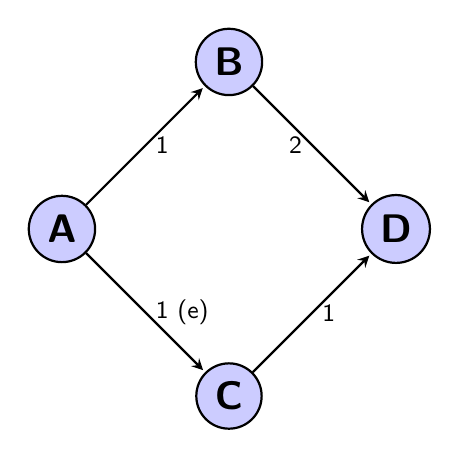
\begin{tikzpicture}[->,>=stealth,shorten >=1pt,auto,node distance=3cm,
 		thick,main node/.style={circle,fill=blue!20,draw,font=\sffamily\Large\bfseries}]

  		\node[main node] (B) {B};
  		\node[main node] (A) [below left of=B] {A};
  		\node[main node] (C) [below right of=A] {C};
  		\node[main node] (D) [below right of=B] {D};

  		\path[every node/.style={font=\sffamily\small}]
    		(B) edge node [left] {2} (D)
    		(A) edge node [right] {1} (B)
        		edge node [right]  {1 (e)} (C)
    		(C) edge node [right] {1} (D);
		\end{tikzpicture}\\
		With edge $e$ as noted (connecting A to C), then $e$ can be part of a min cut.  The max flow of the system is currently 2.  However, if we increase $c(e)$ to 2, then the max flow of the system is still 2, and $e$ is no longer part of a min cut.
	\item $max min(x+y,y+w,3x+w)\\x+y+w=1$
	\item TODO
	\item A is $C(e_I , f(t))$.\\B is $C(f(t), e_I)$.
	\item TODO Assuming $f(x)$ is $O(1)$ and using $n$ to represent the number of intervals, the running time of the above dynamic program is $O(??)$.
	\end{enumerate}
\item Point domination
	\begin{enumerate}
	\item An efficient ($O(n)$) algorithm to find all points of set $S$ which do not dominate any other point in $S$:
		\begin{algorithmic}
		\State $(xlow_x, xlow_y) \gets (\infty, \infty)$
		\State $(ylow_x, ylow_y) \gets (\infty, \infty)$
		\For{$p_i = (x_i , y_i ) \in S$}
			\If{$x_i < xlow_x$}
				\State $(xlow_x, xlow_y) \gets (x_i , y_i )$
			\EndIf
			\If{$y_i < ylow_y$}
				\State $(ylow_x, ylow_y) \gets (x_i , y_i )$
			\EndIf
		\EndFor
		\State $nondominatingpoints \gets [xlow , ylow]$
		\For{$p_i = (x_i , y_i ) \in S$}
			\If{$y_i < xlow_y$ or $x_i < ylow_x$}
				\State $nondominatingpoints \gets [nondominatingpoints, p_i]$
			\EndIf
		\EndFor
		\end{algorithmic}
	\item TODO An efficient algorithm to find the largest subset of points $U \subset S$ where for each pair of points in $U$ neither dominates the other:
		\begin{algorithmic}
		\State \# we define a utility function
		\Function{ylessthan}{$p_i = (x_i , y_i ) , p_j = (x_j , y_j )$}
			\If{$y_i < y_j$}
				\Return 1
			\Else{}
				\Return 0
			\EndIf
		\EndFunction
		\State \# we sort our points by increasing x using mergesort
		\State \# which implementation we omit here
		\State $P \gets mergesort(S)$
		\For{$p_i \in P$}
			\State $U(p_i) = 1 + max\{U(p_i-1 ) + $\Call{ylessthan}{$p_i$, $p_{i-1}$},\\
			\indent\indent\indent\indent\indent\indent$U(p_i-2 ) + $\Call{ylessthan}{$p_i$, $p_{i-2}$}$\}$
		\EndFor
		\end{algorithmic}
	\end{enumerate}
\item Clauses TODO
\item Pattern Subsequences
	\begin{enumerate}
	\item An $O(nm)$ algorithm for finding any occurrence of $s_1$ within $s_2$ with $k$ or fewer mismatched bits:
		\begin{algorithmic}
		\State $matchlocations \gets [ ]$
		\State $i \gets 0$
		\For{$i < n$}
			\State $count \gets 0$
			\State $j \gets 0$
			\For{$j < m$}
				\If {$s_2[i+j] != s_1[j]$}
					\State $count++$
				\EndIf
				\State $j \gets j + 1$
			\EndFor
			\If {$count < k$}
				\State $matchlocations \gets (matchlocations, i)$
			\EndIf
			\State $i \gets i + 1$
		\EndFor
		\State return $matchlocations$
		\end{algorithmic}
	\item TODO An $O(n log n)$ algorithm for any k:
		\begin{algorithmic}
		\State $matchlocations \gets [ ]$
		
		\State return $matchlocations$
		\end{algorithmic}
	\end{enumerate}
\item Sorting by Reversals
	\begin{enumerate}
	\item An absolute lower bound on the number of reversals required to sort a permutation $\pi$ which has $b(\pi)$ breakpoints is $\lceil \frac{b(\pi)}{2} \rceil$.\\
	First, it is not possible to have a list with only $1$ breakpoint.
	\begin{proof}
	If a list $L =$ [$0, \pi_1, \pi_2, ... \pi_n$] had only one breakpoint, it would imply that $\exists \pi_i \in L$ such that $\lvert \pi_{i-1} - \pi_i \rvert = 1$ or $\lvert \pi_{i+1} - \pi_i \rvert = 1$, and $\forall \pi_j \in L, j \neq i, \pi_j = j$.\\
	WLOG, say $\lvert \pi_{i-1} - \pi_i \rvert = 1$ .  This means that the breakpoint is between $\pi_i$ and $\pi_{i+1}$, so either $\pi_i \neq i$ or $\pi_i+1 \neq i+1$.  We must to reverse some portion of the list to attain the state that $\pi_i = i$.  However, we cannot, because $\forall \pi_j \in L, j \neq i, \pi_j = j$, so $i$ is not present elsewhere in the list.
	\end{proof}
	We can resolve at most $2$ breakpoints with a single reversal.
	\begin{proof}
	If we begin with a list $0, \pi_1, \pi_2, ... , \pi_n, n+1$ and we reverse the list between $\pi_i$ and $\pi_j$, then we do not change the number of breakpoints in the segments [$0, \pi_1, ... \pi_{i-1}$], [$\pi_i, \pi_{i+1}, ... , \pi_j$], or [$\pi_{j+1}, ... \pi_n, n+1$].  Either $\rvert \pi_{i-1} - \pi_j \lvert = 1$ or not and either $\rvert \pi_i - \pi_{j+1} \lvert = 1$ or not.  So our possible breakpoint resolutions are 0, 1, or 2.
	\end{proof}
	In the case where a list has three breakpoints, with any reversal we perform, we can resolve at most one breakpoint, thus reducing the problem to the above.
	\begin{proof}
	If a list $L$ has exactly $3$ breakpoints, is of the form $0, 1, ...,i-1, i, i+2, i+3, ... i+j, i+j+1, i+1, i+j+2, i+j+3, ..., n, n+1$.  In this case, we do not want to perform a reversal on any sublist between $0$ and $i$, since those elements are already in order and doing so would introduce a break point.  For the same reason, we do not want to perform a reversal on any sublist between $i+2$ and $i+j+1$ or between $i+j+2$ and $n+1$.  Therefore, we can reverse the list between $i+2$ and $i+j+1$ or between $i+2$ and $i+1$.\\
	In the first case, we create the list $0, 1, ...,i-1, i, i+j+1, i+j, ... i+3, i+2, i+1, i+j+2, i+j+3, ..., n, n+1$, which has $2$ breakpoints.  In the second case, we create the list $0, 1, ...,i-1, i, i+1, i+j+1, ... i+3, i+2, i+j+2, i+j+3, ..., n, n+1$, which has $2$ breakpoints.  Therefore, we can resolve at most one breakpoint with a single reversal in a list with three breakpoints.
	\end{proof}
	In an ideal situation, if $b(\pi)$ is even we could continue resolving $2$ breakpoints until we have $0$ breakpoints, and if $b(\pi)$ is odd we can resolve $2$ breakpoints per reversal until we have $3$ breakpoints (since we cannot have only $1$ breakpoint).  We can then perform a reversal to resolve $1$ breakpoint, leaving us with $2$, and perform the final reversal.\\
	Therefore, the lower bound of the number of reversals needed to resolve $b(\pi)$ breakpoints is $\lceil \frac{b(\pi)}{2} \rceil$.
	\item
	\begin{algorithmic}
	\Function{nextreverse}{$list$}
		\For{$i = 0, 1, ..., n+1$}
			\If{$list[i] \neq i$}
				\State \#find where it is, and if its neighbours follow
				\State choose $j$ such that $\pi_j = i \in list$
				\While{$j < n$ and $\pi_{j+1} - \pi{j} = 1$}
					\State $j \gets j+1$
				\EndWhile
				\Return $\pi_j$
			\EndIf
		\EndFor
		\Return $n+1$
	\EndFunction\\
	\While{ ($i \gets $\Call{nextreverse}{$permutedlist$}) $\neq n+1$}
		\State choose $j$ such that $\pi_j = i \in permutedlist$
		\State $\rho[\pi_i:j]$
	\EndWhile
	\end{algorithmic}
	\end{enumerate}
\end{enumerate}
\end{document}